\documentclass[a4paper]{article}		%Basic Document class: article
\usepackage[english]{babel}			%Babel
\usepackage{url}				%
\usepackage{hyperref}				%Make Links clickable
\usepackage{graphicx}				%For Pictures, includegraphics[options]{name}
\usepackage{fancyhdr}				%For better headers

%%%%%%Setting up the header
\fancyhead{}						% clear all header fields
\chead{\bfseries Medical technology in smart cars}	%Print the ditle of the paper in every header, in the center
\renewcommand{\headrulewidth}{0.4pt}			%Make a line between the header and the content
\pagestyle{fancy}					%Use the fancy style from the package for the headers and footers

%%%%%Edit style of the document

%%%%%Set Title values
\title{									%Set all the data for the title page, which is created later in the document
	
\includegraphics[height=2cm]{images/higlogo}\\\vspace{1cm}	%vspace, vertical space of x cm to the next line
	Medical technology in smart cars\\\vspace{7mm}
	\Large{Project work of group 5}\\\vspace{5mm}			%Large, for a bigger font.
	\normalsize{Spring Semester 2015}\\\vspace{1cm}			
	\large{IMT 3591 Artificial Intelligence\\
		Gj\o{}vik University College
		\\\vspace{1cm}}}

%%%%%%Set author values
\author{			%Set the author, als included on the title page
Laodice Melliti\\
Matr.-Nr: 140159\\
{\tt laodice.melliti@hig.no}
\and 
Jonas Helbig\\
Matr.-Nr: 140165\\
{\tt jonas.helbig@hig.no}
\vspace{1cm}}

%%%%%%%%%%%%%%%%%%%%%%%%%%%%%%%%%%%%%%%%%%%%%%%%%%%%%%%%%%%%%%%%%%%%%%%%%%%%%%%%
%
%Acctual begin of the document
%
%%%%%%%%%%%%%%%%%%%%%%%%%%%%%%%%%%%%%%%%%%%%%%%%%%%%%%%%%%%%%%%%%%%%%%%%%%%%%%%%

\begin{document}	
\maketitle				%Make title page
\thispagestyle{empty} 	%remove the page number
\begin{abstract}		%Short abstract on the title page
	This document is part of our project for the course Artificial Intelligence at Gj\o{}vik University College. This paper describes the architecture and framework of a system which helps elderly and/or people with chronic illnesses, with detection and prevention of potential harmful incidents while driving a car. 
\end{abstract}

\newpage				%Continue on a new page
\tableofcontents		%Generate table of contents
\newpage
%%%%%%%%%%%%%%%%%%%%%%%%%%%%%%%%%%%%%%%%%%%%%%%%%%%%%%%%%%%%%%%%%%%%%%%%%%%%%%%%
%End of title page and Table of contents, the actual content comes
%%%%%%%%%%%%%%%%%%%%%%%%%%%%%%%%%%%%%%%%%%%%%%%%%%%%%%%%%%%%%%%%%%%%%%%%%%%%%%%%
\section{Formal}
Group number: 5\\
Names of the group members: Laodice Melliti, Jonas Helbig\\
Contribution of Laodice Melliti: System 3, Our system, system architecture - graphic\\
Contribution of Jonas Helbig: System 1, system 2, Our system \\
\section{Introduction}
\indent					%Dirty fix, to indent the first line in each section. 
\indent Throughout this paper, we will design an AI system, which could later be implemented in a smart car application. The primary goal of the system is to assist elderly or sick people during everyday driving situations.

We begin this paper with a look at  the state of art in the area of in-car vital parameter monitoring. We give a short overview and look at three systems in more detail. Afterwards, we introduce and describe our proposed system.
\section{State of art}
\indent
\indent Apart from systems designed to prevent drunk driving or systems with eye recognition that detect if the driver falls asleep, there are surprisingly few public used or commercially available systems in the area of in-car vital parameter monitoring. Therefore, we focus here on research done in this area. In \cite{schneider:12}, the authors research on the validation of electrocardiography (ECG) measurement in a car-integrated test framework.

In \cite{eilebrecht:12} the authors describe the relevance of the heart rate variability (HRV), extracted from the ECG, for driver workload detection in real world driving.

In \cite{walter:11} the authors describe the development and testing of a smart cart seat to measure vital signs with non-contact methods.

In the next three sub sections we describe the work in \cite{yamakoshi:07}, \cite{Zocchi:07} and \cite{angelo:10} in more detail.
\subsection{System 1 as described in\cite{yamakoshi:07}}
\indent
\indent In the paper ``A Preliminary Study on Driver's Stress Index Using a New Method Based on Differential Skin Temperature Measurement'' the authors describe the effects of long monotonous driving in a simulated session. Their architecture consists of several sensors that measure different vital parameters like skin temperature, peripheral resistance and normalized pulse volume. As actuators, they use a display for real-time monitoring and they save the data for offline-analysis.
The system itself only measures and presents the data, without taking further actions based on it.
\subsection{System 2 as described in \cite{Zocchi:07}}
\indent
\indent In the paper ``Physiological parameters variation during driving simulations'', the authors use a system of sensors to find correlations between vital parameters like galvanic skin resistance, peripheral temperature and heart rate variability to determine the psychophysical state of the driver. This is especially for sleep attacks and micro-sleeps detections. The architecture consists of several sensors for vital parameter measurement. The actuators consist of a display and several computers to see the data in real-time and to save the data for later analysis. Their long-term goal is to develop a learning agent system which adjusts itself over time to the person usually monitored.
\subsection{System 3 as described in \cite{angelo:10}}
\indent
\indent In the paper ``System for Unobtrusive In-Car Vital Parameter Acquisition and Processing'', the system calculates the driver`s stress level by measuring his vital signs. The sensors are integrated in the car, mainly in the steering wheel. The car displays the results at the driver`s demand and, depending on the results, can adjust the music`s volume and/or block incoming phone call.

\section{Our proposed System}
\indent
\indent Our system, the smart car, is to assist sick and/or elderly people when they need to drive by regularly checking their health.
To do so, we will implement sensors in the car to measure heart rate, blood pressure and skin resistance. By using the gathered data, the car calculates the stress level, the state of consciousness and the general health of the driver. With that, it can warn the driver to, depending on the situation, consider an appointment with a doctor or to call an ambulance. If the driver has too poor health, the car will first ask whether to call for an ambulance or not. If no answer is given, then it will call the ambulance anyway. If, once the call is made, the driver does not talk, the car will send the coordinate using the data from the GPS.
\subsection{PEAS Description}
\paragraph{Performance} The car needs to be able to detect when the driver`s state is harmful for himself and/or other (for example, if the blood pressure is too low there is a risk of losing consciousness) and to warn the driver of his condition.

\paragraph{Environment} For this project, we only consider the driver, the car (which includes all the built in material) and two external devices (heart belt and pressure sensor) which will be further explained in the next paragraph. The environment outside of the car does not influence this system and we assume that the data is not invalidated by the driver`s clothes.

\paragraph{Actuators} We have three actuators. First, a mobile phone which is built in the system. It will call the ambulance if needed. Secondly, speakers that are built in too. We are using the radio speakers. If the driver is listening to it, then the car will overwrite it in case of an emergency. Thirdly, an interface (touch screen) placed next to the radio that can display what the car say.

\paragraph{Sensors} We have three sensors for medical data and two other kinds of sensors. For the medical data, both the blood pressure and the heart beats will be sensed using an external device. We will use a blood pressure meter and a “heart belt” for the heart pressure. Those devices will be put directly against the driver`s skin. As for the skin resistance, we will put the sensors on the stirring wheel. Supposing that the driver drives normally and without gloves, then we can read the data from the tip of the finger (which is the best). The last two sensors are a GPS, either built in the car or from a mobile phone, and the touch screen. The last one is used by the driver to interact with the car (for example when it asks to call for an ambulance).

\subsection{System architecture}
\begin{figure}[h!]
	\centering
	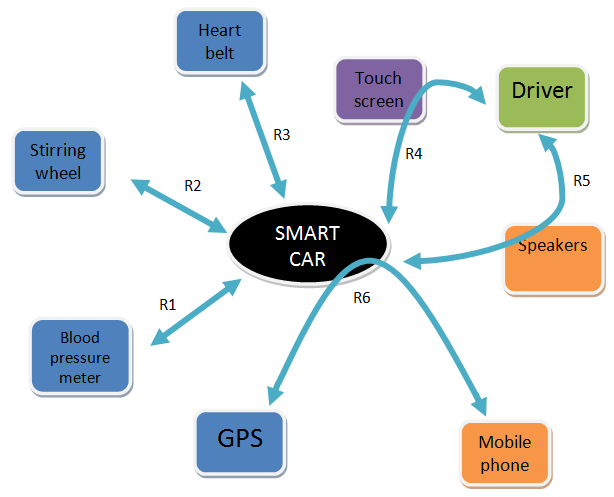
\includegraphics[scale=0.5]{images/architecture}		%Include picture
	\caption{System Architecture}					%Picture caption
	\label{fig:sys}									%Label of the picture, can be referenced with \ref{fig:sys}
\end{figure}
Our system architecture is presented in Figure \ref{fig:sys}.
\begin{description}\addtolength{\itemsep}{-0.5\baselineskip}
	\item{R1:} The blood pressure meter gets the blood pressure’s data (sensor).
	\item{R2:} The stirring wheel gets the data about the skin resistance (sensor).
	\item{R3:} The heart belt gets the data about the heart rate (sensor).
	\item{R4:} The driver gives his answer using the touch screen (sensor \& actuator).
	\item{R5:} The smart car informs the driver of his state using the speakers (actuator).
	\item{R6:} The smart car calls an ambulance using a mobile phone (actuator).
	
	If needed, it uses the GPS coordinates (sensor).
\end{description}
\bigskip
\indent
\indent Our system`s main difference with the other existing project is that we reunite both the capacity to check the driver`s health and the capacity to call someone (here, the ambulance). The combination of this two functionalities has yet to be reunited in the same smart car.
\newpage	%Newpage for the references
%%%%%%%%%%%%%%%%%%%%%%%%%%%%%%%%%%%%%%%%%%%%%%%%%%%%%%%%%%%%%%%%%%%%%%%%%%%%%%%%
%End of the normal document, the Bibliography follows
%The Bibliography is generated from the example.bib file
% ---- Bibliography ----
%%%%%%%%%%%%%%%%%%%%%%%%%%%%%%%%%%%%%%%%%%%%%%%%%%%%%%%%%%%%%%%%%%%%%%%%%%%%%%%%
\bibliographystyle{ieeetr}  	%Set the style for the bibliography, after certain standards
\bibliography{bibliography}			%Automaticly create a bibliography

\end{document}
%End of the whole document, everything from here will be ignored
